\documentclass{standalone}
\begin{document}
	\subsection{Lung Extraction}
	This is a pre-processing step , which involves the creation of a lung mask and the managing of the Hounsfield Unit. The creation of a mask for the lung regions aims to reduce the number of clusters and avoid the formation of false positives by removing external structures, which can be source of errors. In order to achieve this purpose, we have decided to use a pre-trained neural networks~\cite{REP:lungmask} which code is open source. The use of the neural network allows to obtain a good lung segmentation also for patients with severe ILD, from which some lung areas will be excluded with method like threshold and connected components, as we can see in \figurename\,\ref{fig:UNetVSThr}. 
	
	Once we have found a suitable mask for the lung, a managing of HU must be performed. The $k$ constant in the HU definition (equation\,\ref{eq:HU}) may change according to the scan manufacturer or scan model; moreover, during the scan acquisition, all the regions outside the CT tube aren't sampled, so to obtain a square $N\times N$ image for each slice some padding values are added, which different values according to the scan manufacturer: for instance in the CT scan in \figurename\,\ref{fig:Pre-Processing}(a) the padding value is $-3000 HU$ and the air value is $-1024$. 
	
	The first thing to do is to make the padding value and the air value equal for each scan considered and shift them to $1$: in this way we have registered the HU for scan from different manufactures in a common space, as we can see in \figurename\,\ref{fig:Pre-Processing}(b).
	
	 May happen that some patient have metallic prothesis, that lead of HU out of range. Since usually this implant are outside the lung, are removed after the mask application, so no other step are needed.
	 
		\begin{figure}[h!]
		\centering
		\subfigure[Histogram of a CT scan before registration]
		{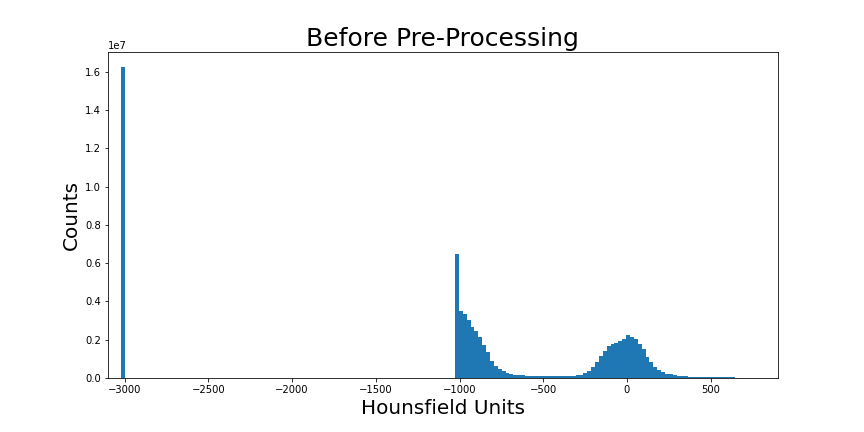
\includegraphics[scale=.3]{HU_before_rescaling.png}}
		%\hspace{1mm}
		\subfigure[Histogram of a CT scan after the registration]
		{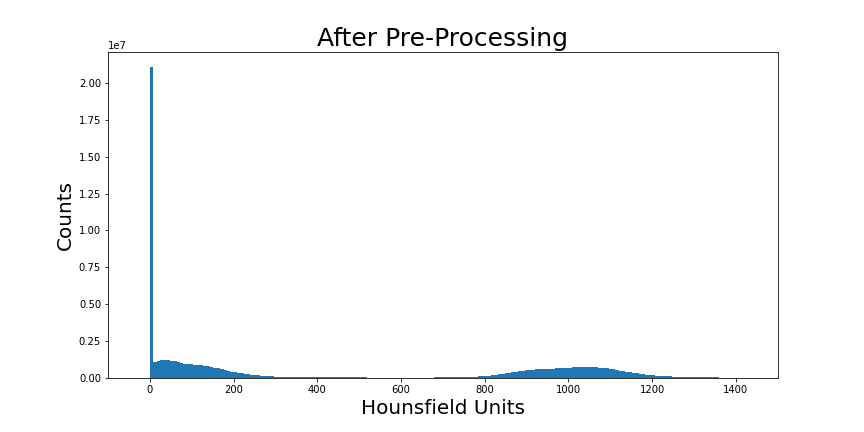
\includegraphics[scale=.3]{HU_after_rescaling.png}}
		\caption{Histogram of voxel values before and after the pre-processing. We can observe that before the pre processing there are some HU out of range, which are the values used to fill the regions outside the tube, and the air value is around $-1000\,HU$ according to HU definition. After the rescaling we can observe that all the values are non-negatives.}\label{fig:Pre-Processing}
	\end{figure}
	Now, we have found the mask for the lung regions, and we have managed the HU, so by a simple element wise multiplication we are able to isolate the lung from the rest of the body, removing also the organs, like heart and intestine, presents in the CT scans.\\
	
	We have observed that the presence of the airpockets and bronchial structure in the lung regions is one of the main source fo false positives, so an extra step was added in order to remove as much as possible this kind of structures.\\ Air pockets have an elongated shape, respect to the other structure which usually are rounded, so the basic Idea was to use this kind of information. By using the \href{https://www.docs.opencv.org/master/dd/d1a/group__imgproc__feature.html#ga04723e007ed888ddf11d9ba04e2232de}{cornerEigenValsAndVecs} function implemented in \textsc{OpenCV}. This particular filter compute the covariant matrix of the derivative in a neighborhood and the corresponding eigenvalues. If a particular regions have an elongated shape, one of the eigenvalues (corresponding to the eigenvector in the direction of the structure) will have an higher values, otherwise both eigenvalues have a lower values. So we have applied this filter on each slice of the scans and took the maximum eigenvalues. 
	\begin{figure}[h!]
		\centering
			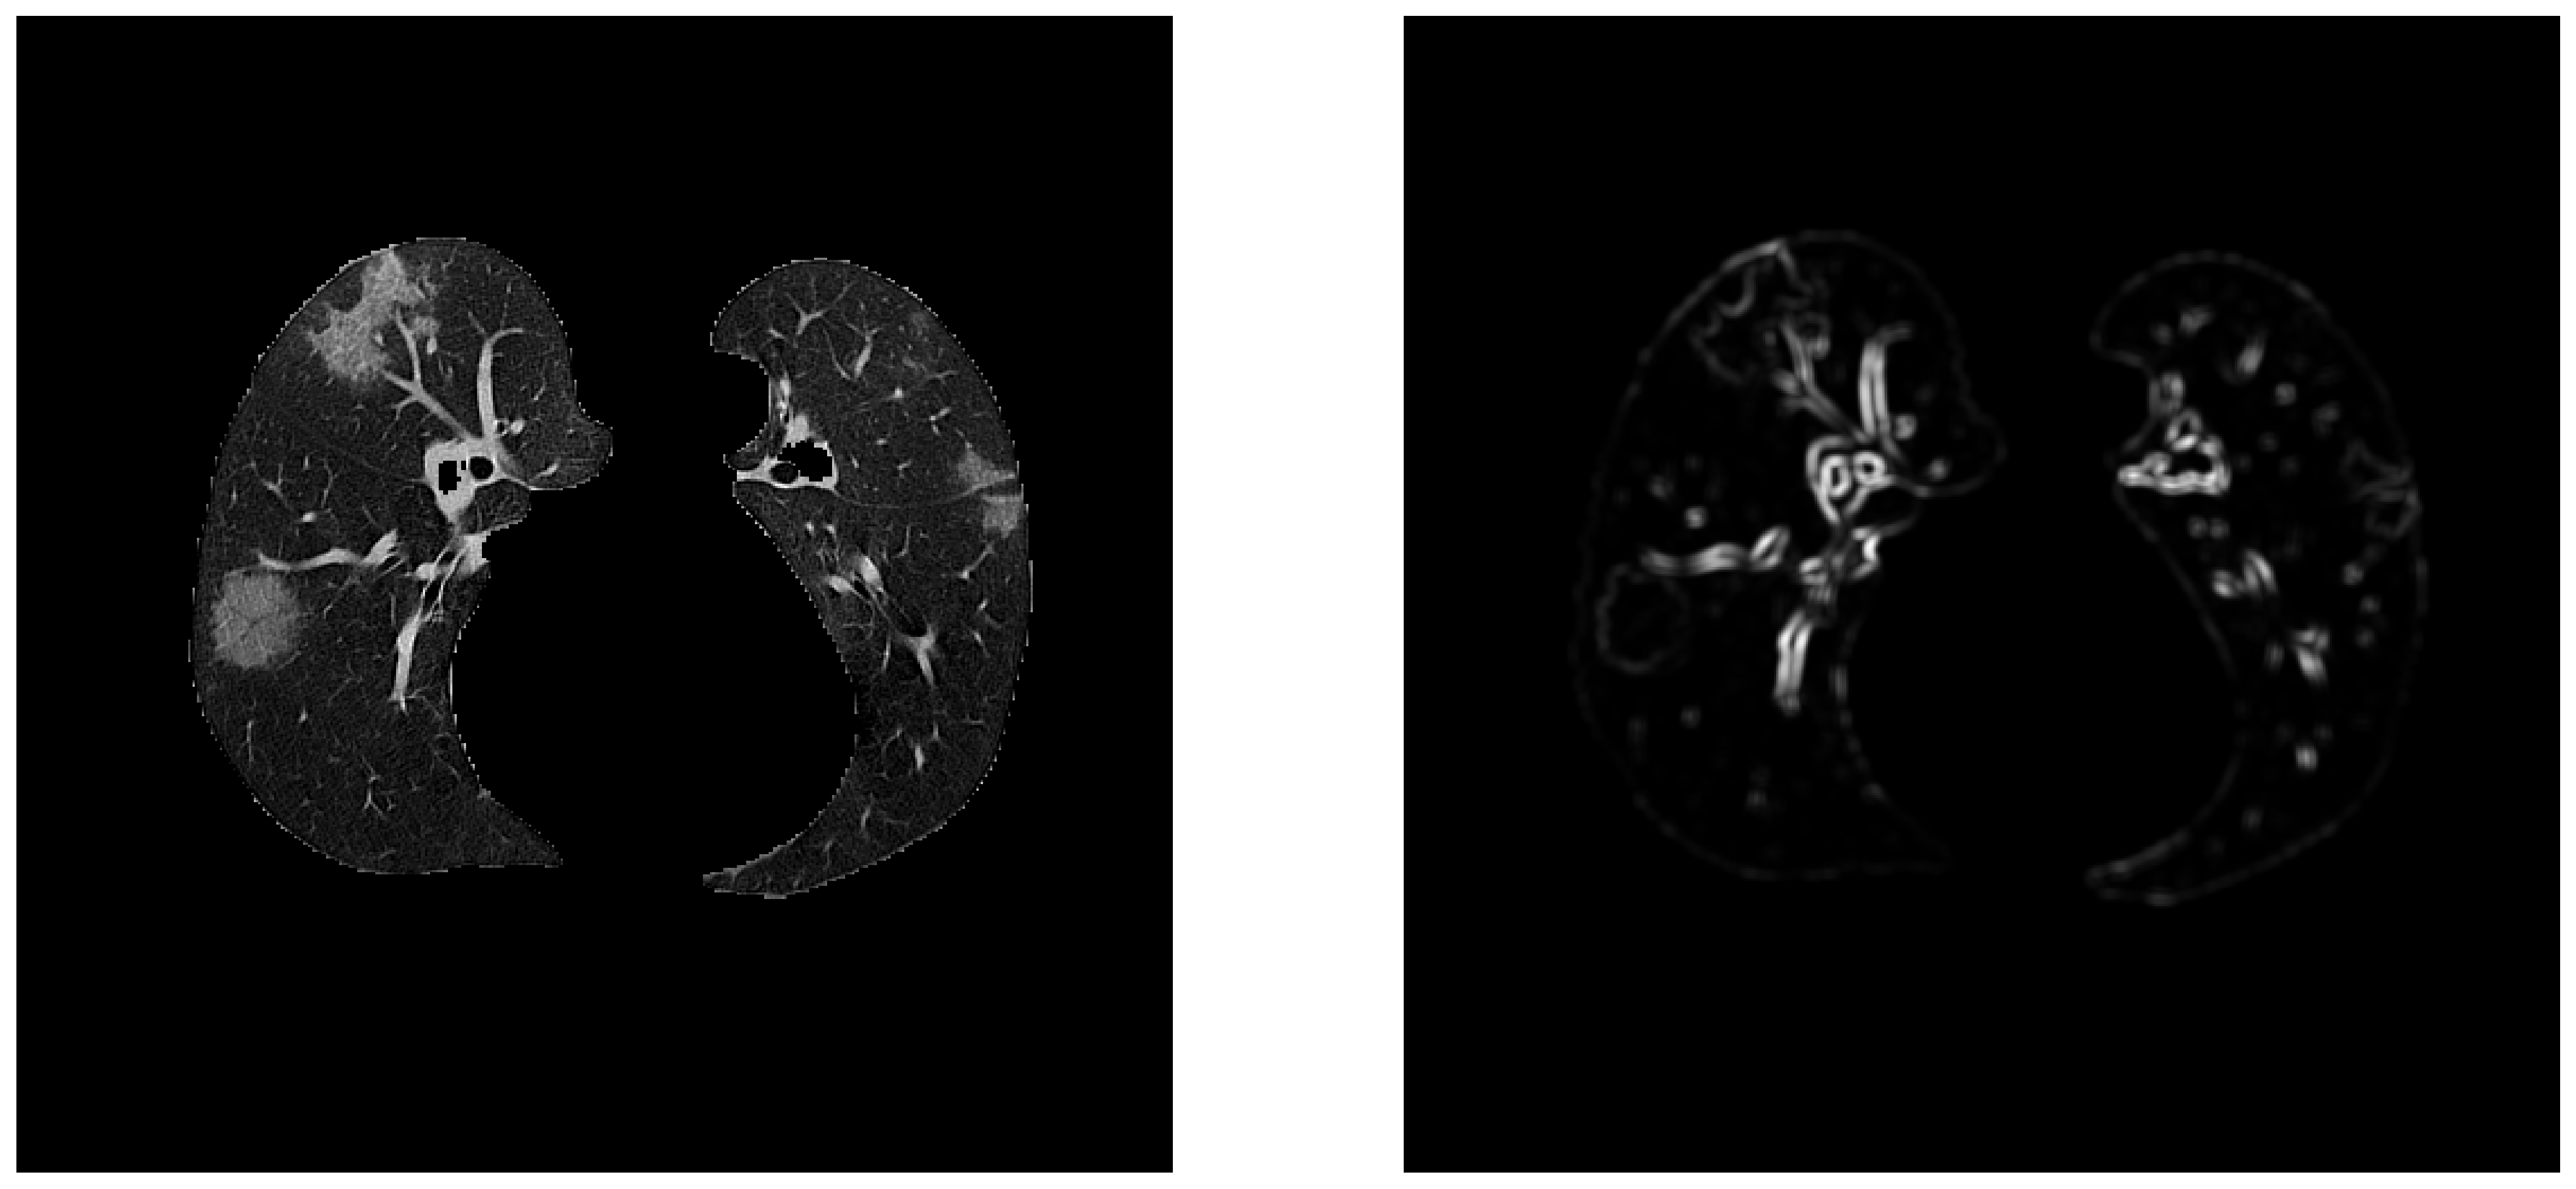
\includegraphics[scale=.3]{MaxEigenVal.png}
			\caption{From left to right: Lung regions selected by the UNet; Maximum eigenvalues map of the lung. As we can see the UNet does not exclude the bronchial structure from the lung, on the other hand, the maximum eigenvalues map delineates very well these regions.We have used this map to remove the unwanted bronchial regions.}\label{fig:MaxEigenval}
	\end{figure}

	In \figurename\,\ref{fig:MaxEigenval}, I've displayed the image after the lung segmentation by the neural network, and the corresponding eigenvalues map. As we can see the higher values of the map corresponds to the edges of the main bronchial structures. To create the mask for these structures a simple threshold on the map was taken. Since the main bronchial structures are large, this process is able to remove only part of the edges, but the inner structure is preserved. In order to refine the segmentation, this process is repeated a second time, allowing a more accurate exclusion of the structures.
		
	Once lung regions are extracted, we are ready to perform the actual segmentation, or, if we haven't already estimate the centroids, performing the training step.\\
	
	
	\begin{algorithm}
		
		\SetAlgoLined
		\DontPrintSemicolon
		\SetKwComment{command}{right mark}{left mark}
		

		\KwData{Volume(CTScan)}
		\KwResult{Volume with extracted lung}\;
		
		mask $\leftarrow$ ApplyUNetModel(Volume)\;
		volume$\leftarrow$ (volume $<\,1200$) = volume air values\;
		volume $\leftarrow$ ShiftMinimumTo1(volume)\;
		lung $\leftarrow\,(volume\circ\, mask)$	\;
		\tcc{Start the bronchial removal}\;
		eigen $\leftarrow$ maxEigenvalues(lung)\;
		alveolar\_mask$\leftarrow$ (eigen $<$ threshold)\;
		lung\_woBronchi $\leftarrow\,(lung\circ\, alveolar\_mask)$\; 
		\tcc{Refine the alveolar removal}\;
		eigen $\leftarrow$ maxEigenvalues(lung\_woBronchi)\;
		alveolar\_mask$\leftarrow$ (eigen $<$ threshold)\;
		lung\_wo\_bronchi $\leftarrow\,(lung\_woBronchi\circ\, alveolar\_mask)$\; 		
		
	\caption{Pseudo-code for the lung extraction script}	\label{alg:lungExtraction}
		
	\end{algorithm}
	
\end{document}